\textbf{مورد استفاده:}
ایجاد پروژه
\\
\textbf{شرح مختصر :UC}
در این قسمت کارفرما پروژه خود را تعریف می‌کند.
\\
\textbf{پيش شرط:}
ورود به داشبورد کارفرما.
\\
\textbf{سناريو اصلی:}
\begin{enumerate}
\item
شروع
\item
کارفرما دکمه ایجاد پروژه را انتخاب می‌کند و سیستم فرم خام را به کارفرما نمایش می‌دهد.
\item
کارفرما فرم را تکمیل می‌کند و با دکمه ارسال، فرم تکمیل شده را به سیستم ارسال می‌کند.
\item
سیستم اطلاعات فرم را بررسی می‌کند و اطلاعات را در بانک اطلاعات ثبت می‌کند.
\item
پایان
\end{enumerate}

\noindent
\textbf{پس شرط:}
ندارد.
\\
\textbf{سناريوهای فرعی:}
\\
\textbf{سناريو فرعی 1:}
خطا در اطلاعات فرم ایجاد پروژه
\\
\textbf{شرح مختصر :UC}
این سناریو در مرحله ۴ سناریو اصلی در صورت خطا در اطلاعات فرم اجرا می‌شود.
\begin{enumerate}
\item
شروع
\item
اطلاعات فرم بررسی می‌شود و خطاها مشخص می‌شوند.
\item
یک پیغام به کارفرما نمایش داده می‌شود و درخواست اصلاح اطلاعات فرم را دارد.
\item
از مرحله 3 سناریو اصلی ادامه پیدا می‌کند.
\item
پایان
\end{enumerate}

\noindent
\textbf{سناريو فرعی 2:}
با موفقیت ثبت شود
\\
\textbf{شرح مختصر :UC}
این سناریو در مرحله ۴ سناریو اصلی در صورت موفقیت‌آمیز بودن ایجاد پروژه اجرا می‌شود.
\begin{enumerate}
\item
شروع
\item
اطلاعات فرم بررسی می‌شود و یک پیغام به کارفرما نمایش داده می‌شود که اطلاعات با موفقیت ثبت شده است.
\item
از مرحله 4 سناریو اصلی ادامه پیدا می‌کند.
\item
پایان
\end{enumerate}

\noindent
\textbf{پس شرط:}
ندارد.


\begin{figure}[H]
	\centering
	\includegraphics[width=1\textwidth]{Diagram/2.Activity/داشبورد-کاربر/کارفرما/ایجاد-پروژه.jpg}
	\caption{دیاگرام فعالیت ایجاد پروژه}
	\label{fig:a:ایجاد-پروژه}
\end{figure}
\begin{figure}[H]
	\centering
	\includegraphics[width=1\textwidth]{Diagram/3.Sequence/داشبورد-کاربر/کارفرما/ایجاد-پروژه.jpg}
	\caption{دیاگرام توالی ایجاد پروژه}
	\label{fig:s:ایجاد-پروژه}
\end{figure}
\begin{figure}[H]
\centering
\includegraphics[width=.8\textwidth]{Diagram/4.Collaboration/داشبورد-کاربر/کارفرما/ایجاد-پروژه.jpg}
\caption{دیاگرام همکار ایجاد پروژه}
\label{fig:c:ایجاد-پروژه}
\end{figure}
